\section{Begriffe}

%TODO Verweise auf die Sektionen

\begin{description}
	\item[aerob/anaerob]\hfill \\
		Abhängigkeit des Stoffwechsels von Sauerstoff.

	\item[Autotrophie] \hfill \\
		\ce{CO2} als Quelle für Kohlenstoff.
		(Auch: Primäproduzenten)

	\item[Chemolithotrophie]\hfill \\
		Energiegewinnung aus Oxidation anorganischer Substanzen.
		Nur bei Prokaryoten.
		(Auch: Chemoautotrophie)\\
		Beispielsweise: \textbf{\ce{H2}} + \ce{O2} \textrightarrow  \ce{H2O} + \textbf{ATP}

	\item[Chemoorganotrophie]\hfill \\
		Energirgewinnung aus Oxidation organischer Stoffe.\\
		Beispielsweise: \textbf{Glucose} + \ce{O2} \textrightarrow  \ce{CO2} + \ce{H2O} + \textbf{ATP}

	\item[Fermentation] \hfill \\
		Anaerober Katabolismus, bei dem eine organische Verbindung sowohl
		Elektronendonator als auch Elektronenakzeptor dient und bei dem
		ATP durch Substratkettenphosphrylierung gebildet wird.

	\item[Glykolyse] \hfill \\
		Ein biochemischer Weg,
		bei dem Glucose fermentiert wird und ATP sowie verschiedenen
		Fermentationsprodukte gebildet werden.
		(Auch: ``Embden-Myerof-Weg'')

	\item[Heterotrophie] \hfill \\
		Abhängigkeit von mehrern Kohlenstoffquellen.
		Zumeist Chemolithotrophe.

	\item[Oxidationsstufen] \hfill \\
		\begin{table}[h!]
		\begin{center}
		\begin{tabular}{l l} 
			\toprule
			Element			&	Summenformel		\\
			\midrule
			\multicolumn{2}{l}{Schwefel}			\\
			Sulfid			&	\ce{S}$^{2-}$		\\
			Sulfit			&	\ce{SO3}$^{2-}$	\\
			Sulfat			&	\ce{SO4}$^{2-}$	\\
			Thiosulfat		&	\ce{S2O3}$^{2-}$	\\
			\midrule
			\multicolumn{2}{l}{Stickstoff}		\\
			Nitrit			&	\ce{NO2}$^{-}$		\\
			Nitrat			&	\ce{NO3}$^{-}$		\\
			\bottomrule
		\end{tabular}
		\caption{Übersicht über die Oxidationsstufen von Schwefel.}
		\label{tab:oxidationsstufen}
		\end{center}
		\end{table}

	\item[oxidative Poshorylierung] \hfill \\
		Bildung von ATP auf Kosten der protonenmotorischen Kraft,
		die durch Elektronentransport erzeugt wird.

	\item[Photophosphorylierung] \hfill \\
		Bildung von ATP durch die protonenmotorische Kraft,
		die durch lichtangetrieben Elektronentransport erzeugt wird.

	\item[Phototrophie]\hfill \\
		Energirgewinnung durch Licht.\\
		Bei der Oxgenen Photosynthese endsteht Sauerstoff als Abfallprodukt,
		bei der Anoxygenen nicht.
		Phototrophe Organismen sind meinst auch Autotroph.
		Licht \textrightarrow ATP

		\emph{Oxygene Photosynthese} wird nur von Cyanobakterien durchgeführt,
		alle anderen Microorganismen betrieben \emph{anoxygene Photosynthese},
		bei der keine Sauerstoff endsteht.

	\item[protonenmotorische Kraft] 	\hfill	\
		Ein energetisierter Zustand der Membran,
		der durch die Trennung von Ladung und den Elelemten des Wassers
		($H^+$ und  $OH^-$) über die Membran endsteht.

	\item[Reduktionspotenzial ($E_0'$)] \hfill \\
		Die einer Verbindung innewohnenden Neigung,
		gemessen in Volt,
		unter Standartbedingungen,
		Elektronen abzugeben.

	 \item[Stoffwechsel] \hfill \\

		\begin{figure}[ht!]
		\leavevmode
		\begin{center}
		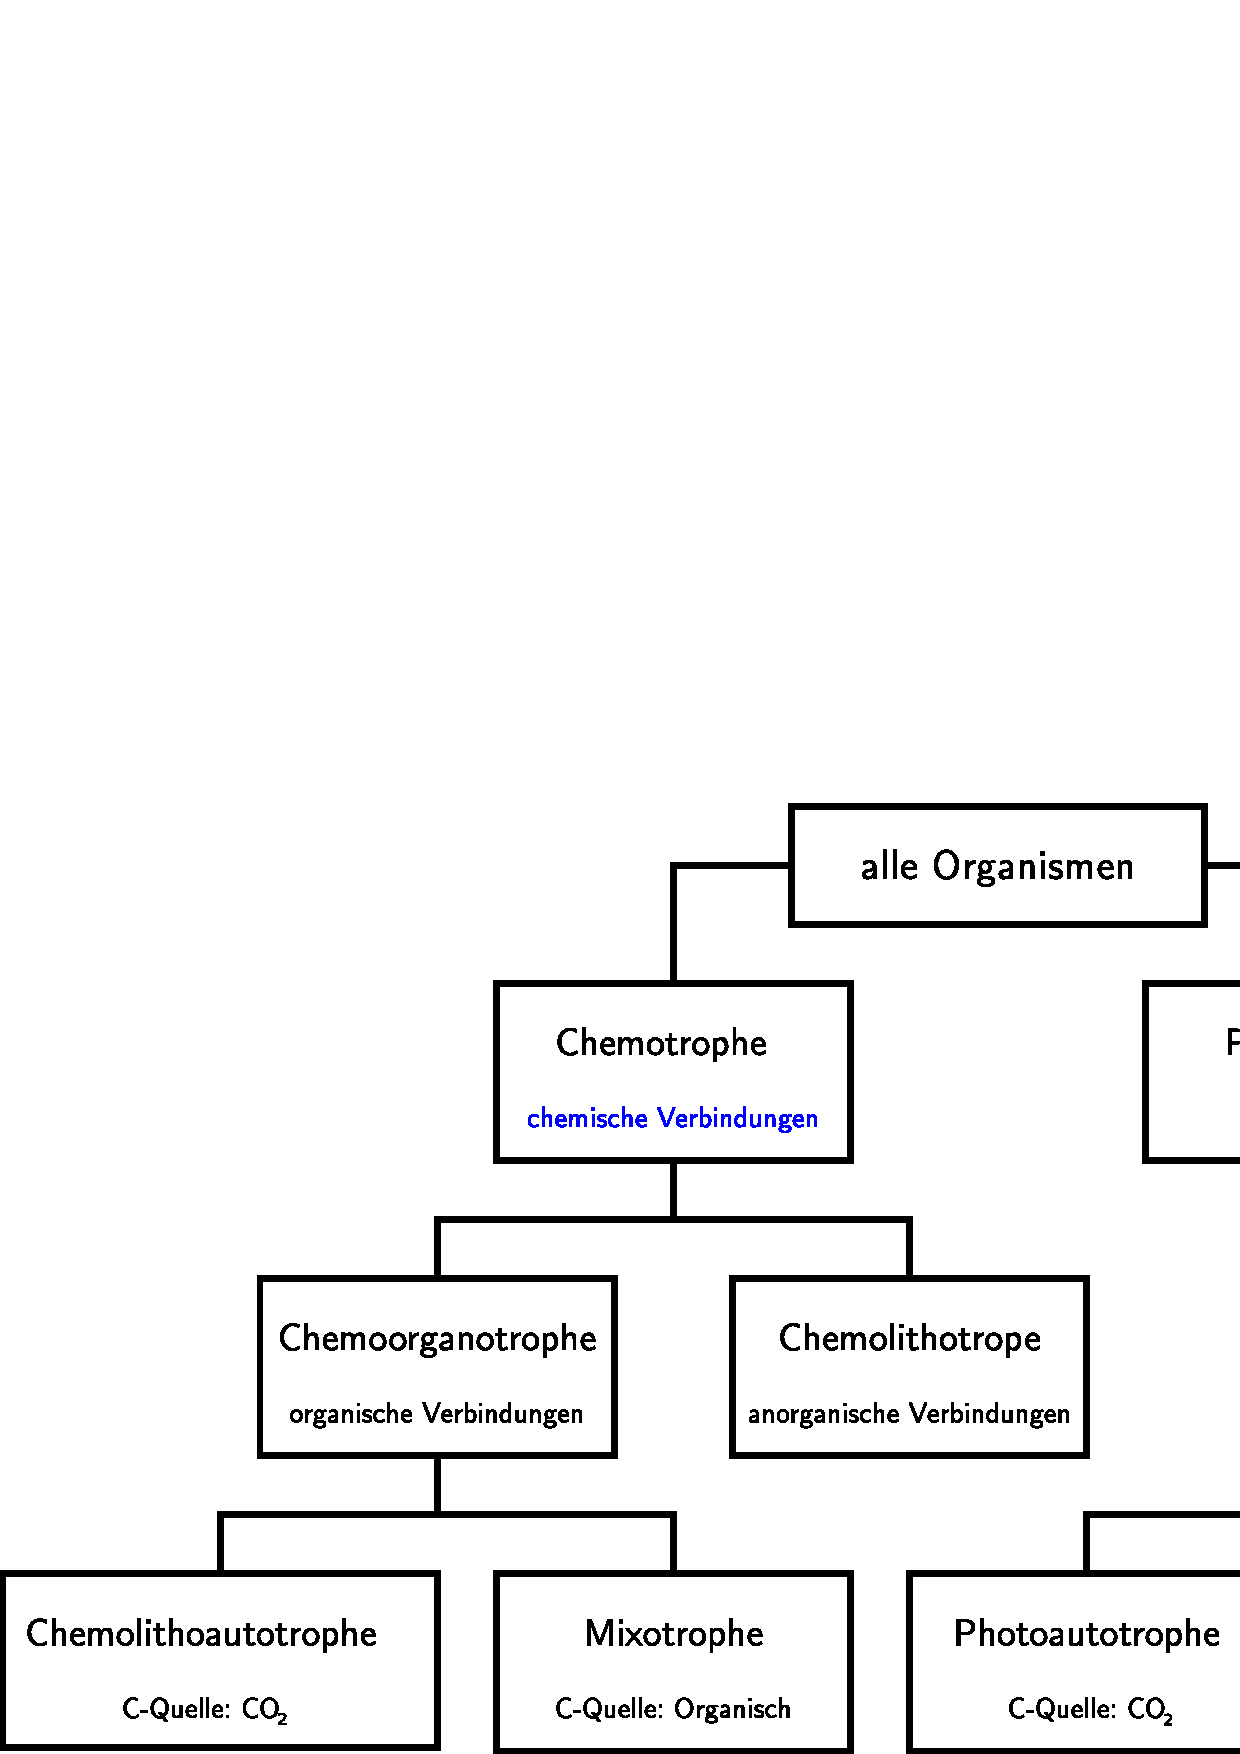
\includegraphics[scale=0.45]{./pictures/stoffwechsel.pdf}
		\end{center}
		\caption{\slshape{Stoffwechselvarianten von Mikroorganismen.
								Dargestellt sind die \textcolor{blue}{Energiequelle} und die Kohlenstoffquelle.}}
		\label{fig:Stoffwechselvarianten}
		\end{figure}

	\item[Substratkettenphosphorylierung]	\hfill	\\
		Bildung von ATP durch den direkten Transfer eines ernergiereichen
		Phosphatmoldeküls von einer phosphorylierten organischen Verbindung
		auf ADP.
		Typisch für Fermentation.
\end{description}
